% !TEX encoding = UTF-8
% !TEX TS-program = pdflatex
% !TEX root = ../tesi.tex
% !TEX spellcheck = it-IT

%**************************************************************
\chapter{Il progetto di stage}
\label{cap:il-progetto-di-stage}
%**************************************************************
\intro{Questo capitolo tratta dettagliatamente delle attività di pianificazione, studio, analisi, progettazione e sviluppo, svolte durante lo stage.}\\




%**************************************************************
\section{Organizzazione}
Per conseguire tutti gli obiettivi fissati, insieme al \emph{tutor} aziendale ho stimato un ammontare di 300 ore. Ho pianificato le attività a monte dello stage in modo modo da distribuire il carico lavorativo in 37.5 ore settimanali, ovvero 7.5 ore giornaliere. In seguito ho rimodulato il piano per focalizzarmi nello sviluppo del modulo Tres.
\subsection{Pianificazione}
Lo stage è cominciato il giorno 5/10/2015 ed è terminato il 27/11/2015. Le attività previste sono state suddivise con cadenza settimanale con questo ordine:
\begin{itemize}
\item \textbf{Prima settimana:}
\begin{itemize}
\item Studio del \emph{database} OrientDB;
\item Studio del linguaggio di programmazione Scala;
\item Studio del \emph{framework} Play;
\item Studio del progetto preesistente;
\end{itemize}
\item \textbf{Seconda e terza settimana:} migrazione dalla tecnologia MongoDB a OrientDB e \emph{porting} all’ultima versione di Play;
\item \textbf{Quarta settimana:} analisi dei requisiti del nuovo modulo;
\item \textbf{Quinta settimana:} progettazione architetturale;
\item \textbf{Sesta e settima settimana:} implementazione modulo;
\item \textbf{Ottava settimana:} test.
\end{itemize} 
%**************************************************************




%**************************************************************
\section{Analisi dei requisiti} 
\subsection{Requisiti}
Per l'analisi dei requisiti ho svolto molteplici incontri insieme al \emph{tutor} aziendale per delineare quali funzionalità dovesse offrire il sistema. Il \emph{tutor} mi ha fornito molti esempi ed illustrazioni per capire al meglio quali requisiti il sistema dovesse soddisfare. Una volta definito le funzionalità ho trascritto i requisiti in un file testuale, in un formato organizzato tabellare. Il file è stato poi sottoposto a versionamento all'interno del \emph{repository} per permettere operazioni di consultazione e modifica all'evolversi dei requisiti. La notazione scelta per suddividere i requisiti è la seguente: 
\begin{center}
R[Importanza][Tipologia][Codice]
\end{center}
\begin{itemize}
\item Importanza può assumere i seguenti valori:
\begin{itemize}
\item \textbf{OBB:} requisito obbligatorio. Il soddisfacimento è necessario per il raggiungimento degli obiettivi dello stage;
\item \textbf{DES:} requisito desiderabile. L'implementazione non è fondamentale, ma
dà valore aggiunto al prodotto.
\end{itemize}
\item Tipologia può assumere i seguenti valori:
\begin{itemize}
\item \textbf{F:} requisiti funzionali. Specifica una funzionalità che il software deve avere;
\item \textbf{V:} requisiti di vincolo. Specifica il vincolo che il software deve avere;
\item \textbf{P:} requisiti di prestazione. Specifica un vincolo di performance che il software deve fornire.
\end{itemize}
\item Codice è un id numerico univoco.
\end{itemize}

Tabella requisiti:
\def\arraystretch{1.8}
\begin{longtable}{|l|p{7cm}|}
\hline
\textbf{Codice} &	\textbf{Descrizione}	\\\hline
ROBBF1	&	Il sistema deve permettere l'inserimento di un nuovo comportamento	\\\hline
ROBBF2	&	Il sistema deve restituire un messaggio di segnalazione in caso di errore durante il salvataggio \\\hline
ROBBF3	&	I dati ricevuti devono essere in formato Json \\\hline
ROBBF4	&	I dati inviati devono essere in formato Json \\\hline
ROBBF5	&	Il sistema deve restituire un messaggio di errore in caso di Json non valido \\\hline
ROBBF6	&	Devono essere inseriti almeno 100 comportamenti per produrre la raccomandazione \\\hline
ROBBF7	&	Il sistema deve restituire un messaggio di conferma quando l'algoritmo è pronto a produrre una raccomandazione	\\\hline
ROBBF8	&	Il sistema deve permettere il calcolo dell'entropia del dataset \\\hline
ROBBF9	&	Il sistema deve permettere il calcolo del guadagno di informazione del dataset	\\\hline
ROBBV10	&	Il sistema deve permettere la costruzione ricorsivamente dell'albero di decisione	\\\hline
ROBBV11	&	Il sistema deve permettere la creazione di tanti nodi quanti sono i possibili valori dell'attributo scelto \\\hline
ROBBV12	&	L'algoritmo di costruzione dell'albero deve fermarsi quando tutte le istanze di un nodo appartengono alla stessa classe \\\hline
ROBBF13	&	Il sistema deve permettere di ricevere una richiesta per classificare un comportamento vuoto \\\hline
ROBBF14	&	Il sistema, per la richiesta con un comportamento vuoto, deve restituire tutte le raccomandazioni con le percentuale calcolate in base al dataset \\\hline
ROBBF15	&	Il sistema deve permettere di classificare un comportamento dell'utente \\\hline
ROBBF16	&	Il sistema deve fornire una raccomandazione o più in base alla classificazione del comportamento \\\hline
ROBBF17	&	Il sistema deve fornire insieme alla raccomandazione la percentuale di adeguatezza	\\\hline
ROBBV18	&	Il sistema deve permettere la modifica dell'albero di decisione ogni 24 ore	\\\hline
ROBBV19	&	Devono essere rispettate le metriche sulla stesura del codice riportate nella sezione 3.6??? \\\hline
RDESF20	&	Devono essere implementati nuovi algoritmi basati sulla teoria de giochi	\\\hline
RDESV21	&	Devono essere implementati nuovi algoritmi di clustering	\\\hline
RDESV22	&	Deve essere sviluppato il pannello di amministrazione	\\\hline
ROBBP23	&	Il database deve essere in grado di memorizzare almeno 100.000 record al secondo	\\\hline
\caption{Tabella dei requisiti}
\end{longtable}
\subsection{Casi d'uso}
In questa sezione riporto i casi d'uso principali. Tres è concepito per operare con Bdrim, una piattaforma di raccolta dati sviluppato in collaborazione con Allos. L'unico attore coinvolto nell'utilizzo di Tres è Bdrim che espone un caso d'uso principale. Per ogni caso d'uso ho specificato gli attori coinvolti, pre e post condizioni, descrizione, scenario principale e se previsto lo scenario alternativo. 
\subsubsection{UC0}
\begin{figure}[h]
\centering
\includegraphics[scale=0.74]{immagini/UC0}
\caption{UC0: Tres}
\label{fig:UC0}
\end{figure}
\begin{itemize}
\item \textbf{Attori:} Bdrim
\item \textbf{Descrizione:} Bdrim usufruisce delle API per ottenere una raccomandazione.
\item \textbf{Precondizione:} Il server è stato avviato.
\item \textbf{Postcondizione:} Il server risponde alle richieste HTTP effettuata dall'utente.
\end{itemize}
\subsubsection{UC1 Revisionare!!!!!}
\begin{figure}[h]
\centering
\includegraphics[scale=0.80]{immagini/UC1}
\caption{UC1: Tres}
\label{fig:UC1}
\end{figure}
\begin{itemize}
\item \textbf{Attori:} Bdrim
\item \textbf{Descrizione:} Questo caso d'uso illustra le funzionalità offerte dalle \emph{API} di raccomandazione a Bdrim.
\item \textbf{Precondizione:} Tres è stato attivato.
\item \textbf{Flusso principale:}
\begin{itemize}
\item[1] Bdrim può richiedere lo stato del sistema;
\item[2] Bdrim può inserire un comportamento;
\item[3] Bdrim può richiedere la raccomandazione.
\end{itemize}
\item \textbf{Flusso alternativo:}
\item \textbf{Postcondizione:} il sistema risponde con una risposta HTTP alla richiesta, ritornando i dati in formato Json.
\end{itemize}
%**************************************************************




%**************************************************************
\section{Progettazione architetturale}
Questa sezione descrive l'attività di progettazione. Illustra l'architettura generale del sistema, le relazioni interne, la struttura del database e infine i \emph{design pattern} utilizzati.
\subsection{Visione ad alto livello}
Il contesto di utilizzo dell'applicativo è la piattaforma di Bdrim. Questa piattaforma permette di gestire nuovi moduli per introdurre nuove funzionalità. Ogni modulo deve essere assolutamente isolato per poter essere facilmente modificabile e interscambiabile con altri moduli che migliorino le sue funzionalità. Quindi la visione generale del sistema si riconduce ad un modello \emph{client-server}
\begin{figure}[h]
\centering
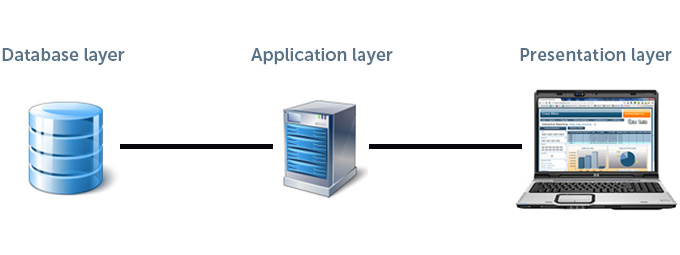
\includegraphics[scale=0.55]{immagini/client-server}
\caption{Visione generale architettura \emph{client-server}. Immagine tratta da \href{http://contentdeliverance.com/2011/client-server-architecture/}{Content Deliverance}}
\label{fig:arch-gen}
\end{figure}

\begin{figure}[h]
\centering
\includegraphics[scale=0.50]{immagini/architetturagenerale}
\caption{Visione generale dell'architettura}
\label{fig:arch-gen}
\end{figure}
\subsection{Architettura}
\subsection{Database}
\subsection{Design pattern}
%**************************************************************



%**************************************************************
\section{Progettazione di dettaglio}
\subsection{Interfaccia}
\subsection{Diagrammi di sequenza}
valutare se utilizzare diagrammi di attività
%**************************************************************




%**************************************************************
\section{Verifica e Validazione}
\subsection{Resoconto risultati}
\subsubsection{Metriche misurate}
Qui di seguito sono riportate le metriche software misurate:
\begin{itemize}
\item \textbf{Complessità ciclomatica:} per il calcolo della complessità ciclomatica ho utilizzato Sbt, al suo interno è disponibile il \emph{tool} styleCheck. Questo strumento segnala con un \emph{warning} se la complessità supera il valore 10. Il \emph{tool} ha restituito esito positivo e non ha segnalato alcun \emph{warning}
\item \textbf{Attributi per classe:} ho rilevato per questa metrica come valore medio 2, mentre come valore massimo ho rilevato 4.
\item \textbf{Copertura commenti:} il valore di copertura è pari al 100\%
\item \textbf{Copertura dei test:} il valore di copertura dei test è del 73\%
\end{itemize}
\subsubsection{Test di unità}
Qui di seguito sono riportati tutti i test di unità eseguiti e il loro relativo esito:
\def\arraystretch{1.8}
\begin{longtable}{|l|p{7cm}|l|}
\hline
\textbf{Test} &	\textbf{Descrizione}	&	\textbf{Stato}	\\\hline
TU1	&	Viene verificato che il sistema salvi correttamente un comportamento all'interno del \emph{database}	&	Esito positivo	\\\hline
TU2	&	Viene verificato il corretto caricamento di una lista di \emph{widgetTag} distinti	&	Esito positivo	\\\hline
TU3	&	Viene verificato il corretto caricamento di una lista di \emph{item} distinti	&	Esito positivo	\\\hline
TU4	&	Viene verificato il corretto caricamento di una lista di \emph{behavior} con una \emph{interaction} specifica	&	Esito positivo	\\\hline
TU5	&	Viene verificato il corretto caricamento di una lista di \emph{behavior} con \emph{tag} e \emph{action} specifici	&	Esito positivo	\\\hline
TU6	&	Viene verificato il corretto caricamento di una lista di \emph{action} distinti	&	Esito positivo	\\\hline
TU7	&	Viene verificato il corretto calcolo dell'entropia	&	Esito positivo	\\\hline
TU8	&	Viene verificato il corretto calcolo del guadagno di informazione	&	Esito positivo	\\\hline
TU9	&	Viene verificato che venga creata la raccomandazione corretta da fornire	&	Esito positivo	\\\hline
TU10	&	Viene verificato il corretto calcolo delle probabilità	&	Esito positivo	\\\hline
\caption{Tabella dei test di unità}
\end{longtable}
\subsubsection{Test di integrazione}
Qui di seguito sono riportati tutti i test di integrazione eseguiti e il loro relativo esito:
\def\arraystretch{1.8}
\begin{longtable}{|l|p{7cm}|l|l|}
\hline
\textbf{Test} &	\textbf{Descrizione}	&	\textbf{Componente}	&	\textbf{Stato}	\\\hline
TI1	&	Viene verificato che il sistema crei correttamente un albero di decisione	&	algorithm	&	Esito positivo	\\\hline
TI2	&	Viene verificato che il sistema aggiorni l'albero di decisione ogni 24 ore	&	algorithm	&	Esito positivo	\\\hline
TI3	&	Viene verificata la corretta creazione del \emph{training set}		&	algorithm	&	Esito positivo	\\\hline
\caption{Tabella dei test di integrazione}
\end{longtable}
\subsubsection{Test di sistema}
Ho effettuato alcuni test di sistema inerenti alle funzionalità di inserimento dati, calcolo di una raccomandazione e infine il calcolo probabilità.
\begin{itemize}
\item \textbf{Inserimento dati:} viene verificato il corretto comportamento del sistema alla richiesta di inserimento dati;
\item \textbf{Calcolo raccomandazioni:} viene verificato il calcolo della raccomandazione da fornire;
\item \textbf{Calcolo probabilità:} viene verificato il calcolo delle probabilità associate ai vari \emph{item}.
\end{itemize}
%**************************************************************
